This chapter describes the system building methodology  \citep{nunamaker1990systems} as applied to deep recurrent architectures for speech recognition.  As this approach involves theory building, system development, experimentation and observation, this chapter describes the procedures which were incorporated in order to achieve the aims and objectives of this research.

In order to arrive at the initial research questions and hypothesis a literature survey  of speech processing advances was carried out.  

The initial research topic was centred around a language learning companion.  Thus, a mini survey was conducted on recipients' use of technology in general learning.  After the literature survey, the research was narrowed down to core language technology assistive features and speech recognition for low resource languages was the chosen area of research focus.

This research develops several software systems based on knowledge acquired from the literature survey in order to gain deeper understanding into the state of the art research results as well as building upon baseline systems in order to achieve the research aims and objectives.  It was through this methodology that the final systems developed in chapters six and seven were designed and developed as a unique combination of existing research systems.  While the system built in chapter seven is a combination of systems in order to generate knowledge in the field of speech recognition, the value added from the system built in chapter six relates to using already successful methods in speech recognition on a new language having linguistic data challenges. 

\section{Assumptions}
This research makes the following assumptions.
\begin{enumerate}
    \item The first assumption is that Software engineering systems are successfully developed using an incremental and iterative manner of increasing complexity.
    \item End-to-end speech models are more conservative on actual software engineering complexity and in that respect are said to be utilised towards low resource speech recognition.
    \item End-to-end speech recognition has been made possible using recurrent neural networks (RNNs) and connectionist temporal classification (CTC) algorithms.
    \item By having a higher number of features, Deep scattering networks (DSNs) can better detect speech than state of the art Mel Frequency Cepstral Coefficients (MFCCs).
    \item There is knowledge to be gained in the application of speech models to new languages.
\end{enumerate}

Based on the above assumptions this research proposes that there is much knowledge to be gained from combining the use of Scatter transform features with RNNs and application of current deep RNNs in the modelling of the Wakirike language.\startblue This knowledge includes among others:
How well does the \acrshort{dsn} features train using an end-to-end approach?
What range of features can be discovered using the \acrshort{dsn} approach?
How fast can we train models using \acrshort{dsn} features in end-to-end \acrshort{asr} modelling.
Are there benefits to be gained by applying sequence models to low-resource \acrshort{asr} systems
\stopblue

\section{Speech Processing software and tools}
This research set out to build and evaluate several speech processing systems.  Some of the systems were built by hand from scratch; however, the end products were adaptations of already existing open source speech recognition research projects.  The systems and platforms adapted for this research include the following:
\begin{itemize}
    \item CMUSphinx
    \item Kaldi
    \item Mozilla DeepSpeech
    \item Scatternet toolbox
    \item Matlab
    \item Tensorflow
    \item Choregraphe
    \item ESPNet
\end{itemize}

While the research sought to focus on speech models for the Wakirike language, several other sub systems were required for but development of the baseline models in addition to the final model the following system development steps were taken to arrive at the final output models:
\begin{itemize}
    \item Auto-correlation experiments
    \item Experiments with Nao robot
    \item CMUSphinx Digits speech recogniser
    \item Digit speech recogniser using Kaldi
    \item Python based speech alignment experiments
    \item Sequence-to-sequence grapheme-to-phoneme (G2P) model
    \item TensorFlow sequence-to-sequence character-to-diacritically-labelled-character model
    \item GRU language model for Wakirike language based on TensorFlow
    \item Bi-Directional LSTM-based end-to-end speech model
    \item End-to-End Speech Network Toolkit (ESPNet) Experiments

\end{itemize}

In the following sections, the tools utilised for the systems developed and how they were utilised is discussed.  Subsequently, the actual systems developed incrementally towards the final models are described.

\subsection{CMUSphinx}
The CMU Sphinx recogniser system is illustrated in Figure \ref{fig_c3_sphinx}.  In a speech application or experiment, the recogniser is called within the user application and is fed with input and other control parameters that determines the recogniser behaviour.  From the illustration, it is observed how the components of feature extraction, acoustic modelling, language modelling and decoding are linked within the CMU Sphinx system.  Note that for identification and clarity classes/modules are capitalised in the following paragraphs.

\begin{figure}
\centering
  % Requires \usepackage{graphicx}
  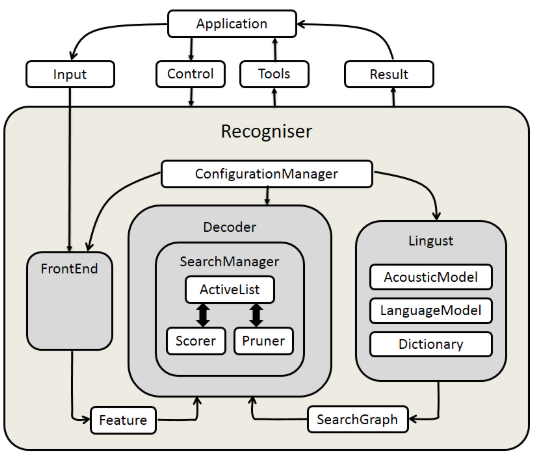
\includegraphics[width=9cm]{thesis/images/sphinx}\\
  \caption{CMU Sphinx4 recogniser system }\label{fig_c3_sphinx}
\end{figure}
In the CMU Sphinx realisation, the \texttt{FrontEnd} module implements feature extraction.  The \texttt{Linguist} module implements the acoustic modelling and the language model component. Finally, the \texttt{Decoder} module implements a decoder.  The \texttt{ConfigurationManager} class is used to determine the behaviour of the recogniser by specifying the parameters of the other modules.   

From this implementation, the \texttt{FrontEnd} processor is the signal processing unit of Sphinx-4 parameterising signals using various implementations into a final sequence of \texttt{Features}.  The \texttt{Linguist} is in charge of language and pronunciation modelling.  This includes phonetic information from the \texttt{Dictionary} and structural information from one or more sets of \texttt{LanguageModel}s and \texttt{AcousticModel}s.  The output of the \texttt{Linguist} is a \texttt{SearchGraph}.  The \texttt{Feature}'s output from the \texttt{FrontEnd} and the \texttt{SearchGraph} output from the \texttt{Linguist} become the input for the \texttt{SearchManager} in the \texttt{Decoder}.  The output of the decoder are \texttt{Results} objects.  At any time prior to or during the recognition process, the researcher can via his application application issue Controls  through the \texttt{ConfigurationManager} to each of the modules, and become a partner in the recognition process.  The following subsections summarise the submodules \citep{walker2004sphinx}.

\subsubsection{FrontEnd Module}
Being consistent with having a ``pluggable'' framework, CMU Sphinx4 has the ability that most of its components can be replaced and at run-time.  This flexibility allows various implementations of the comprising components of the recogniser.  Accordingly, the front end supports but is not limited to \acrfull{mfcc}, \acrfull{plp} and \acrfull{lpc} implementations.  In addition, comprising modules within the various implementations include support for various signal processing utilities such as Hamming Windows, \acrfull{dct}, Bark Frequency Warping, Mel Frequency Filtering, \acrfull{cmn} etc.  All the tasks therefore required by the feature extraction process are implemented in this module.

\subsubsection{Linguist}
The job of the \texttt{Linguist} is to model the higher order and lower order grammar content of the audio input.  This particular module caters for the acoustic model and the language model.  The  various \texttt{Linguist} implementations allow CMU Sphinx-4 to support different tasks such as traditional \acrfull{cfg}, \acrfull{fsgs}, finite-state transducers and small N-gram language models.  This module has three pluggable modules representing the \texttt{Dictionary}, \texttt{LanguageModel} and \texttt{AcousticModel}.  The \texttt{Dictionary} comprises the pronunciation of all the words to be used in the \texttt{Decoder}. Sphinx-4 Linguist provides primary support for the CMU Pronouncing Dictionary (Carnegie Mellon University, 2016). The \texttt{SearchGraph} produced by the Linguist is capable of sharing parameters such as Gaussian mixtures, transition matrices and mixture weights and Sphinx-4 provides a single Acoustic model supporting acoustic models generated by the Sphinx-3 trainer.  Depending on the memory architecture various implementations of the Linguist include the \texttt{FlatLinguist}, \texttt{DynamicFlatLinguist} and \texttt{LexTreeLinguist}.  These will either create the \texttt{SearchGraph} entirely in memory or on demand.  Finally, the \texttt{LanguageModel} supports a variety of formats such as \texttt{SimpleWorldListGramar} which as the name implies supports a simple word list.  The \texttt{JSGFGramar} is a BNF-style platform-independent realisation of the Java Speech API Grammar format. \texttt{LMGrammar} produces a bigram model. \texttt{FSTGrammar} supports finite-state transducer ARPA FST grammar format. The \texttt{SimpleNGramModel} support N-gram model and the \texttt{LargeTriGramModel} is suited to optimise memory storage.

\subsubsection{Decoder}
Provides a pluggable \texttt{SearchManager} to simplify decoding.  \texttt{Decoder} tells \texttt{SearchManager} to recognise a set of \texttt{Feature} frames. This creates a \texttt{Result} object that contains all the paths that have reached a final non-emitting state(i.e. Word endings).  Applications can modify the search space and Result object between steps, permitting the application to become a partner in the recognition process.  The \texttt{SearchManager} is not restricted on any particular implementation, examples include Frame synchronous Viterbi, Bushderby, A*, bi-directional and parallel searches.

Each \texttt{SearchManager} uses a token passing algorithm described by (Young, Russel & Thornton, 1989).  A sphinx-4 token is an object that is associated with a \texttt{SearchState} and contains the overall acoustic and language scores of the path at a given point, a reference to the \texttt{SearchState}, a reference to an input \texttt{Feature} frame, and other relevant information.

The \texttt{SearchManager} sub-framework generates \texttt{ActiveLists} from currently active tokens in the search trellis by pruning using a pluggable Pruner. These in turn can be modified by the application to perform both relative and absolute beam pruning.

The \texttt{SearchManager} sub-framework also communicates with the \texttt{Scorer}, a pluggable state probability estimation module that provides state output density values on demand.

\subsubsection{Other modules}
\texttt{ConfigurationManager} allows various module implementations to be combined in various ways.  Finally, we illustrate how the \texttt{ConfigurationManager} creates Automatic Speech Recognition (ASR) experiments using the CMU-sphinx4 objects described above in the sample program from \cite{Lamere03thecmu} 
\begin{lstlisting}[language=Java,basicstyle=\small]

package com.example;
import java.io.File;
import java.io.FileInputStream;
import java.io.InputStream;

import edu.cmu.sphinx.api.Configuration;
import edu.cmu.sphinx.api.SpeechResult;
import edu.cmu.sphinx.api.StreamSpeechRecognizer;

public class TranscriberDemo {                                  
    public static void main(String[] args) throws Exception {      
        Configuration configuration = new Configuration();
        configuration
        .setAcousticModelPath("resource:en-us");
        configuration
		  .setDictionaryPath("resource:cmudict-en-us.dict");
        configuration
        .setLanguageModelPath("resource:en-us.lm.bin");

        StreamSpeechRecognizer recognizer = new StreamSpeechRecognizer(
                configuration);
        InputStream stream = new FileInputStream(new File("test.wav"));

        recognizer.startRecognition(stream);
        SpeechResult result;
        while ((result = recognizer.getResult()) != null) {
            System.out.format("Hypothesis: %s\n", result.getHypothesis());
        }
        recognizer.stopRecognition();
    }
}
\end{lstlisting}
The above java code sample represents a user application.  We see three classes being imported. The \texttt{Configuration}, \texttt{SpeechResult}, and \texttt{StreamSpeechRecognizer} class.  The \texttt{Configuration} object holds resources for the acoustic model, language model and phonetic dictionary.  The \texttt{SpeechRecognizer} object has different implementations representing the source of the speech signal.  In the above sample the \texttt{StreamSpeechRecogniser} class is used to load the speech signal from a wave (.wav) file.  However other speech signal sources are available such as the \texttt{LiveSpeechRecogniser} which implements loading the speech sound signal from a microphone device if available.  In addition, \cite{walker2004sphinx} 4 asserts that the Sphinx-4 system provides additional tools and utilities that contain helper classes for computing recognition statistics such as Word Error Rate (WER), phoneme error rates (PER) etc.

\subsection{Kaldi}
CMU Sphinx provides an object-oriented approach to speech recognition. Kaldi \cite{povey2011kaldi} on the other hand is a highly modularised library written in C++. Kaldi is based on weighted finite state transducers (WFSTs) used for inference graphs and decoding. The Kaldi WFSTs utilises OpenFst, an open source library, at its core. Together with a collection of configuration scripts for building complete recognition systems, Kaldi supports modeling of a variety of speech model variations with vast support for linear and affine transforms of speech features of arbitrary phonetic-context sizes.  Kaldi is specifically suited for acoustic modeling with subspace Gaussian Mixture Models (SGMM) in addition to the standard Gaussian Mixture Models (GMMs).
\subsubsection{Architecture}
The component architecture of Kaldi is illustrated in the figure below.  Modules can be divided into those that utilise the linear algebra libraries and those that use OpenFST.  The decodable class forms the link between these two scopes.  The rest of the modules lower down the hierarchy are based on modules higher up hierarchy according to this divide.
\begin{figure}
\centering
  % Requires \usepackage{graphicx}
  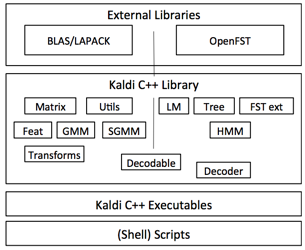
\includegraphics[width=9cm]{thesis/images/kaldi}\\
  \caption{Kaldi Architecture\citep{povey2011kaldi}}\label{fig_c3_kaldi}
\end{figure}
\subsubsection{Feature Extraction}
Kaldi supports various speech feature outputs including the standard \acrfull{mfcc}, \acrfull{plp}, \acrfull{vtln}, \acrfull{cmvn}, \acrfull{lda}, \acrfull{stc},\acrfull{mllt}, \acrfull{hlda}.  These systems are made complete with various configuration parameters for fine tuning their individual models.
\subsubsection{Acoustic Modelling}
Full co-variance as well as diagonal co-variance GMM modelling is implemented in Kaldi. Efficient log-likelihoods are computed using simple dot products of mean times in-variance and in-variance co-variance.  The \texttt{DiagGmm} class is responsible for storing co-variances of Gaussian densities. The Acoustic Modelling (AM) class represented by the \texttt{AMDiagGmm} class comprise a set of \texttt{DiagGmm} objects.  These objects which represent Gaussian Mixture Models (GMMs) are in turn represented Probability Density Function (PDF) indices which are then mapped to \acrfull{hmm} states. There are classes to represent HMM topology as well as the overarching topology representing transition modelling. These two sets of classes provide information required for developing decoding graphs.  Rather than using the conventional approach for HMM modelling using hand-made decision tree for left and right phones in a mono-phone model, tree-clustering algorithms automatically generate the decision tree.

\subsubsection{Language Modelling and Decoding Graphs}
Using the \acrfull{fst} back in addition to third party language modelling software, Kaldi is able infer sentence estimations using n-gram language models. During decoding, transition-ids are created and attached to corresponding pdf-IDs as a result of tied-state nature of phones where different phones are allowed to have share the same distribution.  The transition-id therefore encapsulates the shared pdf-ID and the arc (transition) of phone-specific topology. This way transitions are fine-grained without adding complexity to the decoding graph

Core decoding algorithms are implemented using C++ classes one per decoder.  Decoders implement an interface which accepts an acoustic model score for a particular input-symbol and frame.  While single-pass decoding is achieved through C++ classes, multi-pass decoding is realised using the supporting configuration scripts.

\subsection{Mozilla DeepSpeech}\label{sec_c3_moz}
The DeepSpeech speech-to-text engine is an ASR speech model and model generator built by Mozilla is based on Baidu's Deep Speech research paper \citep{hannun2014deep}.  The system comes in two forms;  an installable speech-to-text engine based on the English language and the model trainer. These components were created and run effectively on Unix based systems and to a limited extent on Microsoft Windows systems.  Various options for installing the speech to text engine includes either command line based or as an application programming interface (API) using python or NodeJS.  In addition, the speech-to-text (STT) engine API also supports bindings for the Rust language, GoLang and GStreamer.  This thesis however, did not rely on the STT engine nor API, but rather on the model trainer which was adapted in this research for scattering transform feature-based end-to-end speech recognition.

Runtime library dependencies of both the STT engine and the model trainer include libsox, 2 for sound processing of audio; libstdc++6, libgomp1 and libpthread are used to compile the Connectionist Temporal Classification (CTC) decoder implementation which incorporates the KenLM trained language model \citep{Heafield-estimate}.
\subsubsection{Graphics Processor Unit (GPU)-Enabled Speech Model Training}
The model trainer of the Mozilla DeepSpeech platform is facilitated by the ability to train models on a highly parallel processing Graphics Processing Unit (GPU).  This enables model training-time speed-ups over traditional CPU machines.  The Mozilla DeepSpeech platform recommends Nvidia Graphics 10 series processor with a system requirement of 8GB of Random Access Memory (RAM). In section \ref{sec_c3_tf} we introduce TensorFlow python library.  Mozilla DeepSpeech platform is able to utilise the GPU using the Nvidia GPU library, CUDA.  This is achieved through the python TensorFlow library created by Google as discussed in section \ref{sec_c3_tf}.
\subsubsection{Common Voice training}
The speech corpus used for training in this research was obtained from the Mozilla Common Voice Initiative speech corpora.  This consists of over 250 hours of speech data that is subdivided into test, development and training data sets.  In addition, the data was subdivided into clean data, that is, clean audio recording with accurate translation and a small subset containing skewed data, that is, audio recording which was either noisy or lacking accurate transcriptions.  The skewed data subset consisted 15-25\% of the training corpus and was incorporated so that the neural network speech model could simulate and learn real world noisy audio speech-to-text translation.  The Mozilla DeepSpeech model trainer provided bash scripts for importing the Common Voice speech corpora as well as converting the files into the appropriate formats and provision of mapping files for the model trainer.
\subsubsection{Mozilla DeepSpeech model parameters}
The model trainer consists of a root python script ``DeepSpeech.py'' with various calls to other python scripts responsible for things like audio processing, distributed training, GPU configuration, training coordination.  Other accessory bash scripts also present are responsible for downloading and training for different kinds of speech corpora including Mozilla Common Voice\citep{mozilla/deepspeech_2019} and the Wall Street Journal (WSJ)\citep{paul1992design}.  These sets of scripts are referred to as speech corpus importers. 

In order to supply the model trainer with a set of hyper parameters for tuning various aspects of the Mozilla DeepSpeech platform, the following categories arguments passed to the root script ensue:
\begin{itemize}
    \item Geometry - Defines the number of neurons in the hidden layers of the neural network.
    \item Cluster configuration - Parameters responsible for distributed training of the speech model across various nodes.
    \item Global constants - These include all other parameters to gain fine control of the training process.  These parameters include how much of the training corpus will be used and which subset should be included; early stopping for pre-trained models that have already been trained to saturation, that is to a stopping condition; the dropout rate for neural network regularisation.  This is a strategy to overcome over-fitting where instead of learning inference features the data, the neural network memorizes the training data.
    \item Global constants - These include all other parameters to gain fine control of the training process.  These parameters include how much of the training corpus will be used and which subset should be included; early stopping for pre-trained models that have already been trained to saturation, that is to a stopping condition; the dropout rate for neural network regularisation.  This is a strategy to overcome over-fitting where instead of learning inference features the data, the neural network memorizes the training data.
    \item Adam optimiser - parameters for the Adam optimiser
    \item Batching - set the number of batches during training.
    \item Weight Initialisation - standard deviation coefficients for initialising weights.
    \item Checkpointing - this includes the number of seconds before saving the current model parameter values to the disk.  This enables resumption of training in instances where the training was interrupted. For training to resume successfully, the resuming training geometry parameter must be exactly the same as the interrupted geometry training parameter.
    \item Exporting - Includes parameters for saving a saturated model for inference.
    \item Reporting - Includes options for setting the log-level however reports are only sent to the standard console output.
    \item Decoder - These parameters include the path to the alphabet symbols and that of the custom CTC decoder used during decoding of the neural network output.
    \item Inference - It is possible to use a model trainer to either perform a one-shot inference or resume training from an already exported model. The parameters used for inference are responsible for performing these stated tasks.
\end{itemize}

In addition to the above configuration there are other accessory scripts that can be used for TensorFlow specific tasks such as conversion of the output model graph to several exportable formats.

\subsection{Matlab and ScatNet toolbox}
In this research, feature processing of audio files to obtain their deep scattering transforms was achieved using a MATLAB toolbox known as ScatNet \citep{anden2014scatnet}.  The ScatNet toolbox in general analyses time-series sampled analog signals and has been used successfully for music genre classification, texture and image classification \citep{anden2011multiscale,sifre2013rotation,sifre2014rigid}.  In particular, the scattering transforms produced are signal processing layers of increasing width where each layer constitutes the convolution of a linear filter bank wavelet operator (Wop) with a non linear complex modulus.  
\begin{equation}
    ||\text{complex signal}|\star \mathbf{Wop}|\star(\text{low-pass filter}) \label{eqn_c3_scat00}
\end{equation}

It is the scattering transforms of the audio files that were fed into the DeepSpeech model trainer discussed in Section \ref{sec_c3_moz}.  The architecture of a scattering networks resembles a deep convolutional network in the sense that each subsequent layer is a mapping of all possible paths from the previous layer.

ScatNet provides default options for most of the parameters that require tuning in order to derive the scattering coefficients for an input signal.  In particular, for audio signals, the most important hyper-parameters set by the library is the number of scattering layers that captures the entire audio spectrum which is set at 2.  In addition to this default, the only other parameter to set is the window period of the signal to be analysed per time.  A suitable value for the window can be derived from the sampling rate of the input signal.  The toolbox function \texttt{S=scat(x,Wop)} takes a an input signal, \texttt{x},  and an array of linear wavelet operators, \texttt{Wop}, in order to compute the scattering coefficients of the input signal.   The resulting network, \texttt{S} is a cell array whose length $M+1$ is equivalent to that of the linear filter operator.  

\subsubsection{Wavelet Factories}\label{sec_c3_scat00} 
By providing optimal defaults for linear operators, ScatNet provides wavelet factories especially suited for efficient signal processing of images and sounds.  Therefore, linear wavelet operators are built in a single command function through built-in “factories”, which perform wavelet analysis tasks.

Further, the maximum number of wavelets $J$ is automatically derived from the sampling from the sampling period $T$.  The filter banks are formed by dilating the mother wavelet ($\psi$) by the dyadic factor ($2^{1/Q}$).  In the Fourier domain this is expressed as
\begin{equation}
     \hat\psi_j(\omega) = \hat\psi(2^{j/Q}\omega)
     \label{eqn_c3_scat01}
\end{equation}
For audio application, to ensure optimized frequency coverage without frequency-redundancy or overlapping, the mother wavelet $(\psi)$ is chosen so that  $(Q_1 = 8)$ and $(Q_2 = 1)$ by default. This also means that the first order filter will be of a higher frequency resolution when compared to the second order filter. 
\subsubsection{Filter banks}\label{sec_c3_scat01}
In order to visualise the filters being used by the wavelet operations and referring to Sections (\ref{sec_c5_wproof} and \ref{sec_c7_wparams}) where it is shown that the first and second order scattering coefficients are respectively defined by the following forms
\begin{equation}
    S_1x(t,j_1) = |x\star\psi_{j_1}|\star\phi(t)
    \label{eqn_c3_scat02}
\end{equation}
\begin{equation}
    S_2x(t,j_1,j_2) = ||x\star\psi_{j_1}|\star\psi_{j_2}|\star\phi(t) \label{eqn_c3_scat03}
\end{equation}
where $(\psi_{j})$ are band-pass filters and $(\phi)$ is  a low-pass filter.

Furthermore, the wavelet transform operators(Wop) created by the wavelet\_factory\_1d function are only function handles and do not have any data in themselves. A second return value may be retrieved from the wavelet factory which contains the set of filters returned as a cell array by the wavelet factory.
\begin{verbatim}
    [Wop,filters] = wavelet_factory_1d(N, filt_opt);
\end{verbatim}

The filters return argument has a similar structure to the scattering network where each element in the cell array corresponds to the layer order in the scatter network hierarchy. Moreover, similar to the the scatter network, the filters cell array hierarchy has $M+1$ elements, where only $M$ elements are utilised and no filters exist at $M=0$. The non-zero coefficients of the band pass filters expressed in the Fourier domain, are held in \texttt{filters{m}.psi.filter} field. When plotting these filters, they are first padded with zeros to the length of \texttt{N} which is the entire spectrum.  Below is the sample plot made against default filters obtained by the \texttt{wavelet\_factory\_1d} filter.

The script below calculates filter banks at orders $(M = 1)$ and $(M = 2)$.  The resulting plot is displayed in Figure \ref{fig_c3_wplot}.

\begin{lstlisting}[language=Matlab]
figure;
for m = 1:2
    subplot(1,2,m);
    hold on;
    for k = 1:length(filters{m}.psi.filter)
        plot(realize_filter(filters{m}.psi.filter{k}, N));
    end
    hold off;
    ylim([0 1.5]);
    xlim([1 5*N/8]);
end
\end{lstlisting}

\begin{figure}
\centering
  % Requires \usepackage{graphicx}
  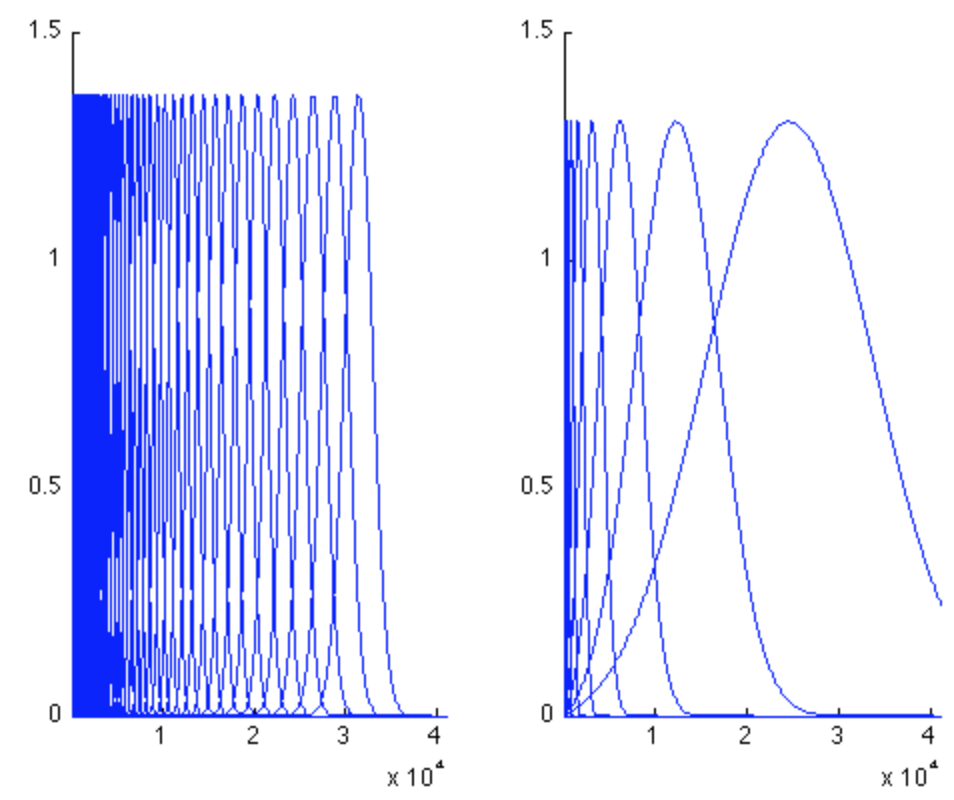
\includegraphics[width=9cm]{thesis/images/wfplot}\\
  \caption{Scatter transform wavelet filters}\label{fig_c3_wplot}
\end{figure}

\subsubsection{Using the Matlab API}\label{sec_c3_scat02}
In the previous sections it was seen how the ScatNet toolbox calculates scatter coefficients based on wavelet theory.  In this section, the scattering spectrum of an audio signal is implemented using only three command calls to ScatNet library.

The three steps taken in this section are as follows.  First load the audio file and set the properties of the audio file required for audio processing of the signal within ScatNet.  Note that to do this the sampling rate of the input signal is required. Here, a clip of Handel’s Messiah, implemented in Matlab as a function is loaded into a “y” variable by default with the “load handel” command.

Given that the sampling rate of the loaded clip is , the parameters set are 
\begin{enumerate}
    \item N - the number of samples in the signal, and  
    \item T - the window size.  Here, T is set to 4096 which corresponds to about half a second.
\end{enumerate}
\begin{verbatim}
    load handel;	% loads the signal into y
    N = length(y);
    T = 2^12;   	% length of the averaging window
\end{verbatim}

The second step is to create the filter operators for which the type of filter signal length, and the window length are passed in as parameters.  It has been shown in the preceding sections that two layers are sufficient to capture energy contained in an audio signal and by default the quality factors of the two layers are $(Q_1 = 8)$ and $(Q_2 = 1)$. These default\_filter\_options are automatically integrated with the 'audio', filter type option.
\begin{verbatim}
    filt_opt = default_filter_options('audio', T);
    Wop = wavelet_factory_1d(N, filt_opt);
\end{verbatim}
Note that the wavelet\_factory\_ functions is an intensive operations because many filters are being built at once  in batch processing of signals discussed in Section \ref{sec_c3_sbatch}, we therefore only perform this as part of the initialisation and the returned wavelet operators (Wop) can be reused without having to recreate them.

Having all the parameters required, in the third and final step , call the scattering transform of y generic function scat, to derive the scatter coefficients.
\begin{verbatim}
    S = scat(y, Wop);
\end{verbatim}

\subsubsection{Scatter Feature Enhancements and Batch Processing}\label{sec_c3_sbatch}
Having obtained the scatter coefficients, further feature enhancement is achieved by taking the log of the normalised coefficients.  This can be visualised using the  built-in scattergram function which produces a translation-invariant, second-order, spectrogram-like visualization of the  scattering transform a one-dimensional audio signal. 

In the code snippet below, \texttt{j1} is the second-order coefficients arbitrarily chosen to equal \texttt{23}.  The first parameter to scattergram are the first-order coefficients and the second wildcard [] parameters gathers all paths from the first order.  
\begin{verbatim}
    j1 = 23;
    scattergram(S{2},[],S{3},j1);
\end{verbatim}

\begin{figure}
\centering
  % Requires \usepackage{graphicx}
  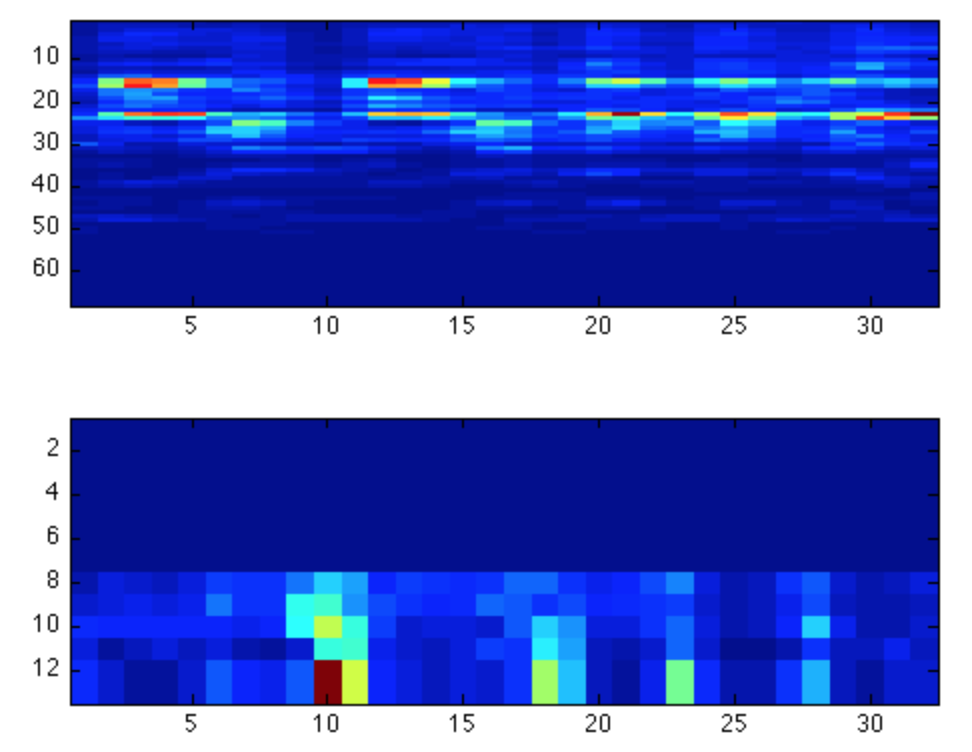
\includegraphics[width=9cm]{thesis/images/wscat0}\\
  \caption{Unnormalised scattergram}\label{fig_c3_sgram00}
\end{figure}

The following functions in the code snippet below are applied to realise the log of the normalised scattergram.
\begin{verbatim}
    S = renorm_scat(S);
    S = log_scat(S);
    scattergram(S{2},[],S{3},j1);
\end{verbatim}

\begin{figure}
\centering
  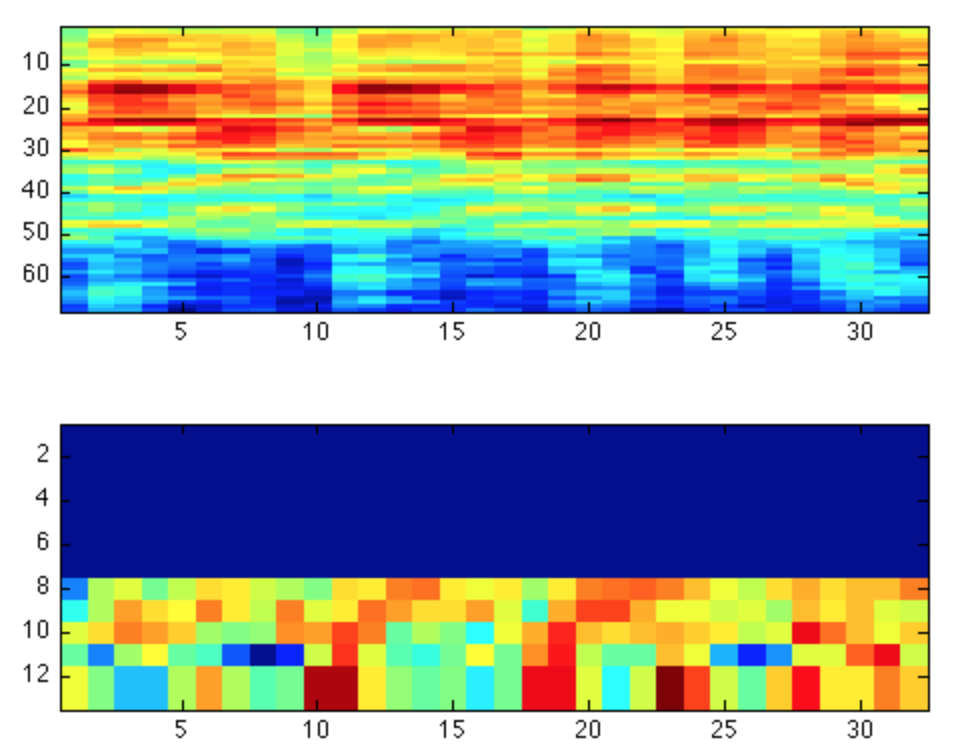
\includegraphics[width=9cm]{thesis/images/wscat1}\\
  \caption{Log normalised scattergram}\label{fig_c3_sgram01}
\end{figure}

With the corresponding scattergram illustrated in figure \ref{fig_c3_sgram01}.

Finally, to utilise the scattering coefficients as features for classification tasks, we extract the vector form using \texttt{format\_scat} function.
\begin{verbatim}
    [S_table, meta] = format_scat(S);
\end{verbatim}

The \texttt{S\_table} is a P-by-N table, where \texttt{P} is the flattened total of all the scattering combined coefficients within each layer of the \acrfull{dsn} and \texttt{N} is the number of time points. The network is now feature ready for classification tasks using an affine space classifier.

For batch processing ScatNet provides a database feature which can accept a collection of input vectors rather than a single input signal.  The following commands show ScatNet commands for performing batch processing on the GTZAN dataset used for musical genre classification

First, specify the path to the audio target.
\begin{verbatim}
    src = gtzan_src('/path/to/dataset');
\end{verbatim}

Next all the defaults for ScatNet analysis and processing are set as explained in the previous Sections \ref{sec_c3_scat00},\ref{sec_c3_scat01} and \ref{sec_c3_scat02} above.
\begin{verbatim}
    N = 5*2^17;
    T = 8192;
    filt_opt.Q = [8 1];
    filt_opt.J = T_to_J(T, filt_opt);
    scat_opt.M = 2;
    Wop = wavelet_factory_1d(N, filt_opt, scat_opt);
    feature_fun = @(x)(format_scat( ...
    log_scat(renorm_scat(scat(x, Wop)))));
\end{verbatim}

It is possible to optimise the training by sub-sampling each signal.  The feature\_sampling option is used to specify sub-sampling.
\begin{verbatim}
    database_options.feature_sampling = 8;
\end{verbatim}


Finally, a call is made to \texttt{prepare\_database} function to compute all the scatter network features of the \texttt{src} database.
\begin{verbatim}
    database = prepare_database(src, feature_fun, database_options);
\end{verbatim}

In this research, further speed up was achieved by utilising Matlab’s parallel processing on the for loop (see Appendix III) thus bypassing the batch processing utility of ScatNet.

\subsection{TensorFlow}\label{sec_c3_tf}
TensorFlow is a state-of-the-art high performance library by Google for Deep learning.  Deep learning is a branch of artificial intelligence which acquires learning from deep neural network architectures.  The paragraphs and subsections that follow under this topic give an overview of the TensorFlow library as outlined by the following authors \cite{goldsborough2016tour,abadi2016tensorflow} and \cite{abadi2017computational}.

Deep learning has significantly advanced in various application domains and by far out-performed traditional approaches.  TensorFlow offers researchers and enthusiasts an open source software library for use in defining, training and deploying deep learning models.

TensorFlow works by defining data flow graphs with mutable state.  A data flow graph represent complex functional node and edge architectures, where each node represents an operator instance applied to input values which constitutes the edges. The operators are implemented by abstract kernels for particular types of interchangeable devices (such as CPUs and GPUs)\citep{abadi2017computational}.

There are three main concepts at TensorFlow's core.  These concepts are tensors, operations and mutability.  Tensors are arrays of arbitrary dimensions where the underlying data type is either specified or inferred at graph-construction time. Operations process data and constitute nodes within the compute graph. Basic operations invariably are mathematical functions such as vector dot products.  However, some of the operations indeed may be associated with a read or state update. Such tensor which permit run-time updates in TensorFlow are referred to as variables.  Finally, there may be edges for communicating and constrain the order of execution. These structures invariably affect the observable graph semantics and may also affect the computation performance. 

Once a TensorFlow program constructs a graph using a client interface such the Python API, the TensorFlow program can send messages to the graph, by “feeding” it inputs and “fetching” outputs from it. TensorFlow then propagates the input values through the execution graph performing  operations called by the client code, until all nodes instructed to run returned with their outputs. 

Data dependencies and control edges, dictate the order of execution. Often, a graph is executed severally and tensors declared as placeholders or constants are used once. However, variable tensors have mutable state which allow persistence across multiple executions. The parameters of the model stored in variables are usually updated as part of running the graph.

\subsubsection{Programming Model}
In this section examples of execution data flow graphs are given; and in the following sections we highlight the other major special features of TensorFlow including automatic differentiation and back-prop algorithm implementation, control flow, check pointing, programming interface, sample implementation and graph visualisation.

In a TensorFlow computational data flow graph, vertices or nodes of the directed graph represent operations, while edges signify flow of data between these vertices or operations. Thus labels on nodes are representative of the actions taken at that node.  Similarly, labels representing values flow in the direction of the edges. The inputs to a labeled operation are therefore the labels which have edges directed towards the operation. A computation or data flow graph is illustrated in Figure \ref{fig_c3_tfg}. 
\begin{figure}
\centering
  % Requires \usepackage{graphicx}
  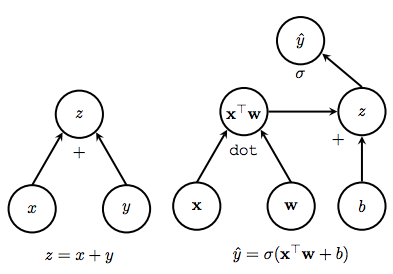
\includegraphics[width=9cm]{thesis/images/tfgraph}\\
  \caption{Sample TensorFlow computation graphs\citep{goldsborough2016tour}}\label{fig_c3_tfg}
\end{figure}

The left graph displays a basic compute graph consisting of an addition operator having two input variables $x$ and $y$.  The result, $z$ is the output of the $+$ operation.  The right graph gives an example logistic regression function. $\hat{y}$ is the final output of the function for some sample vector $\mathbf{x}$, weight vector $\mathbf{w}$ and scalar bias $b$.  As shown in the graph, $\hat{y}$ is the output of the sigmoid or logistic function $\sigma$

\subsubsection{Backprop nodes}
The Backprop algorithm \cite{Goodfellow-et-al-2016} is an efficient method to compute error values for weights within a multilayer or deep neural network.  The algorithm is summarised as follows.  Assuming a neural network with two hidden layers. The two layers within the network respectively have output functions $f(x;w)$ and $g(x;w)$ such that $f(x;w)=f_x(w)$ and $g(x;w)=g_x(w)$.  Where $x$ is the input from the previous layer or from the input layer and  are the weights.  The error function , is an implicit function of all the previous layers.  In the case of the 2-layer network $e=(f_x \circ g_x)(w)=f_x(g_x(w))$.  The back prop algorithm uses the chain rule to correctly assign appropriate updates to each weight at every layer within the network.  The updates which are the gradient or the error function with respect to the weights are $de_x/dw$. The backprop algorithm therefore uses the formula $[f_x(g_x(w))]'=f'_x(g_x(w))\cdot g'x(w)$ as it traverses the graph in reverse to compute the updates. 
\begin{figure}
\centering
  % Requires \usepackage{graphicx}
  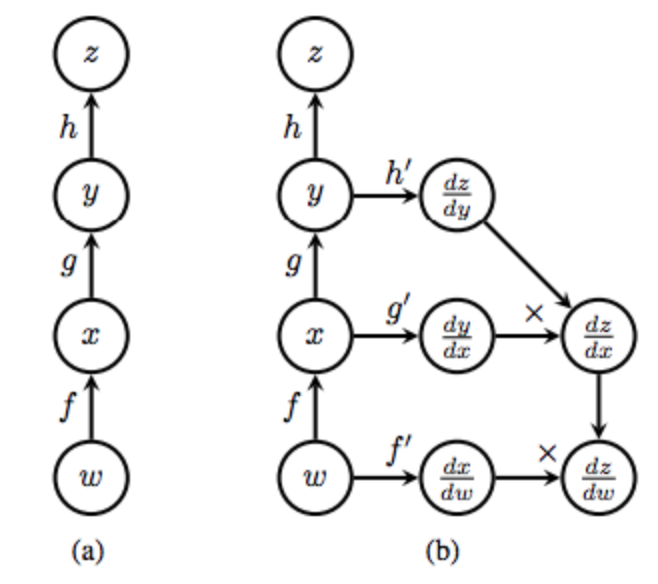
\includegraphics[width=9cm]{thesis/images/bprop}\\
  \caption{Tensorflow graph with backprop nodes \citep{goldsborough2016tour}}\label{fig_c3_bprop}
\end{figure}

Figure \ref{fig_c3_bprop} illustrates how tensor implements backprop by adding two extra nodes at the appropriate layers within the network to satisfy the chain rule.  For each operation encountered, there is a corresponding gradient function that reverses the output as a function of the inputs.  The output of this gradient function can then be propagated backwards to a previous operation which would represent a previous layer within a neural network.  The gradient function propagated to the previous layer is then used to complete the parameters of the chain rule by multiplying with that previous layer’s gradient.  This output is ready to be propagated down the network to the subsequent layer to perform a similar function.  This process continues until all the weights within the network have appropriate update values.

\subsubsection{Control flow}
TensorFlow also supports control-flow operations.  For this reason TensorFlow is not a directed acyclic graph (DAG) but can support cyclic structures. If the number of loops required by the computation graph is known at graph construction.  It is easy to maintain a DAG structure simply by unrolling the number of loops specified.  However, this is not always the case.  There are instances in which a variable number of loops is required at runtime.  Hence, the computation graph becomes increasingly complex.  This is particularly the case for back gradient descent and back propagation of errors (see section \ref{sec_c3_tfw} for a  walk through).  The process of stepping back through a loop in reverse to compute gradients is known as back-propagation through time \citep{al2016theano}.

\subsubsection{Checkpoints}
One can add Save a node to a compute graph, connecting them to variables whose tensors can then be serialized. At another instance one may connect the same variable to a Restore operation. This operation deserializes the stored tensor at another point within the execution graph. This is especially useful over long periods of training to keep track of the model’s variable parameters. These elements form part of distributed TensorFlow's fault tolerance ecosystem.

\subsubsection{Programming Interface}
TensorFlow implementation provides two developer interfaces which include the Python interface and the C++ interface.  While the python interface offers a rich feature set for creation and execution of computation graphs, the C++ interface is primarily a back end implementation with a much more limited API primarily used for executing graphs built with Python and serialised to Google’s protocol buffer.

It is worth noting that unlike PyTorch \citep{ketkar2017introduction}, the Python API handshakes very well with NumPy\citep{numpy} numeric and scientific open source programming library. As such, TensorFlow tensors can be naturally substituted with NumPy ndarrays without any need for type-conversion seen in PyTorch tensors.

\subsubsection{Tensorflow client model walk through}\label{sec_c3_tfw}
In this section, a sample client tensorflow model is examined. The model consists of a simple multi-layer perceptron (MLP) with one input and one output layer to classify hand-writtin digits in the MNIST\citep{krizhevsky2012imagenet} dataset.   In this dataset, the examples are small images $28 \times 28$ pixels depicting handwritten digits from $0$ to $9$.  The examples form a matrix having the shape $\mathbf{X}\in\mathbb{R}^{n\times 784}$ where  represents the number of images, and 784 represents the flattened 28 x 28 pixel image.  The client code performs an affine transform operation, $\mathbf{X\cdot W+b}$, where $\mathbf{W}$ is the matrix of weights $\in \mathbb{R}^{784 \times 10}$, and $\mathbf{b}$ is a vector of biases  $\in R^{10}$.  The result of the affine transform operator is the matrix $\mathbf{Y}\in \mathbb{R}^{n\times 10}$. The resulting non-probabilistic logits gives an unnormalised distribution of digits.In order to obtain the valid probability distribution $Pr[x=i]$ where $x$-th example is classified as the digit $i$, the soft-max method is utilised. 
\begin{equation}
softmax(\mathbf{x})_i=\frac{\exp(\mathbf{x}_i)}{\Sigma_j\exp(\mathbf{x}_j)}\label{eqn_c3_smax00}
\end{equation} 

Error loss values are then computed using an objective function and the model’s current training parameters $\mathbf{W}$ and .  This is obtained from the cross entropy calculation given by
\begin{equation}
    H(\mathbf{L,Y})_i=−\Sigma_j\mathbf{L}_{i,j}\cdot\log(\mathbf{Y}_{i,j})
\end{equation}

Where $\mathbf{Y}=softmax(\mathbf{x})$ and $\mathbf{L}$ are the correct one-hot-encoded labels.  More precisely, the batch-mean loss over all inputs $\mathbf{x}$.


Next, the \acrfull{sgd} is run to update the weights of our model.  A TensorFlow class is provided and will be initialised with a learning rate.  The minimise function of this class takes the loss tensor as parameter used for minimisation.

The operations run repeatedly within a \texttt{tf.Session} context manager. Refer to Appendix IV for the complete code listing.

\subsubsection{Visualisation}
TensorFlow interface offers the option of visualising computation graphs. Complex topologies consisting of various sub-layers can be presented in a lucid form, offering the user a congruent, organised picture of exactly how data is consumed in a compute graph. Sub-graphs may be grouped into visual blocks and referred to in name scopes.  For example a single neural network layer may take up such a named scope. The name scopes are then interactively expanded on to give the detailed group visualisation.

Two types of metrics are obtainable from the TensorBoard. These are summary operations, when attached as nodes in the graph, permit the user to monitor individual tensor values over time.   The first is the scalar summaries which capture tensor values and can be sampled at certain points within training epochs. One can now, for example, observe the trend of the accuracy loss of the training model over time.

The other summary operation offers the user the ability to track distributions, such as final soft-max densities or the distribution of neural network weights. 

Lastly, sample images can be visualised on the TensorBoard graph. This way kernel filters of a convolutional neural network can also be visualised.  In addition to all of these, one can perform zooming and panning actions directly on TensorBoard's web interface including expansion and collapsing of individual name scopes

\subsection{Choregraphe}
The Choregraphe software tool is a high-level language used for programming of Nao humanoid robots.  This is built on top of the Naoqi/Gentoo Unix/Robot Operating System(ROS) \citep{pot2009choregraphe}.  Speech recognition and processing modules of the Choregraphe tool were explored and expanded at the initial stages of the research.  However the Choregraphe software tool for the Nao robot was found to be unsuitable in speech recognition at the level of research that aligned with the research objectives and therefore was not utilised in this work.

\subsection{Alisa}\label{sec_c3_alisa}
Alisa tool is a lightly supervised sentence segmentation tool based on Voice Activity Detection (VAD) algorithms \citep{stan2016alisa}.  It is so called lightly supervised because it requires small amounts of training data.  Generally the tool was asserted to be optimised for sentence segmentation and offered assistance in the creation of new speech corpora in a language-independent fashion. 

The Alisa tool researchers deploy a two-step method for aligning speech, and claim performance up to 70\% imperfect transcriptions often found in online resources can be successfully aligned with a word error rate of less than 0.5\%.  This tool is therefore said to be suitable for development multilingual and under-resourced language aligned speech-corpora.

The motivation behind Alisa was to reduce the time and effort used to gather large amounts of quality data as well as actively eliminate the domain knowledge required to phonetically transcribe speech data.  In addition, and as a bonus to achieving the first objective, is the ability to migrate speech technology fairly seamlessly from one language to another and therefore realise the rather tedious task of automatic transcription of a new language.

\subsubsection{Alisa Architecture}
The goal of automatic transcription of new language with low resource constraint is particularly valuable to this research and as such, it would be relevant to review the enhancements introduced to Alisa.  The two step-method consists of a GMM-based sentence level segmenter and also an iterative grapheme acoustic model used for alignment.  The sentence level GMM-based speech segmenter is used to automatically segment speech into utterances which as discussed earlier forms the basic unit of processing within any ASR system.  This attempts to relieve the researcher off the manual process of segmenting the continuous audio file manually. This process included a GMM-based voice activity detector trained from about 10 minutes of manually labeled data. The second step grapheme based acoustic model is supplemented with a highly restricted word network they referred to as a skip network.  Together an iterative acoustic modelling training procedure is formulated.  The method described required the initial training data and a minimal labelling procedure that involved simple letter to sound rules and inter-sentence silence segments to provide an orthographic transcript of the initial 10 minute recording data.  Therefore, this process is resource-effective because non-experts can also provide this data.  The actual alignment process made use of a grapheme level Viterbi decoder to drive the iteratively self-trained grapheme models.  The model architecture is shown in the figure below.
\begin{figure}
\centering
  % Requires \usepackage{graphicx}
  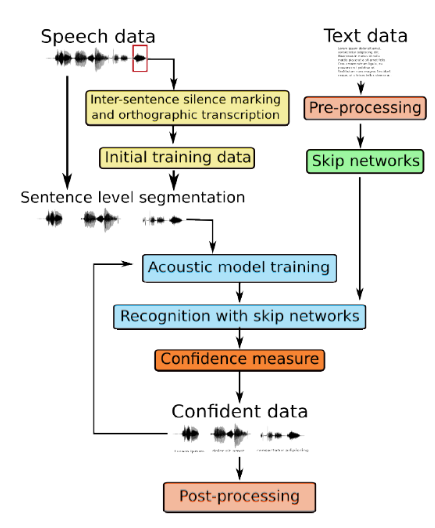
\includegraphics[width=9cm]{thesis/images/alisa}\\
  \caption{Alisa Architecture\citep{stan2016alisa}}\label{fig_c3_alisa00}
\end{figure}

Figure \ref{fig_c3_alisa00} shows a block diagram of the steps involved in the alignment.  The method can be applied to any language with an alphabetic writing system, given the availability of speech resource and its corresponding approximate script.

There is an option of using a grapheme based acoustic model. This however increases the margin for error.  Several steps were introduced in the Alisa tool to minimise this error margin. The chief being the introduction of a tri-grapheme acoustic model which is modeled after using context dependent triphones in traditional acoustic modelling.  Other techniques deployed to crash the error margin include the use of discriminative training with the Maximum Mutual Information (MMI) criterion \citep{schluter2001model} and methods described in \citep{novotney2009analysis}. It was observed that Alisa provided good alignment but was not fully featured. For instance it had no way of adding insertions and substitutions in the audio data not provided in the transcription.  Finally, Alisa was found to be restricted to only languages that can utilise the English alphabet.

\section{Pilot Studies}
The experiments in the following sections describe initial experiments based on the initial study of a language learning companion before the research was narrowed down to a low resource speech recognition.  These preliminary experiments in addition to a preliminary Language Learning Survey helped to narrow down the Research to the specific speech processing task of Low Resource Automatic Speech Recognition (LR-ASR).

The following sections describe analysis of raw wave-forms using auto-correlation signal processing in Matlab and experiments made with the Nao robot speech processing engine and experiments with speech recognition toolkit and speech processing tasks.  These tasks include digit recognition systems using CMUSphinx and Kaldi speech recognition toolkits and speech alignment tasks using the Alisa tool.

\subsection{Auto-correlation Experiments}\label{sec_c3_corr}
Preliminary experiments were carried out on raw speech signals in an attempt to quickly segment individual phonemes based on a basic threshold algorithm.  Further experiments designed an auto-correlation algorithm to attempt to discover a phoneme alphabet in a particular data set in a semi-supervised fashion.
 
\textcolor{blue}{This method had the goal of simulating posterior distributions of phonemes from auto-correlation estimates.  This presents an unnormalised posterior distribution measurement of phoneme segments over the entire signal.  Note that this was a pilot study, as such, the data used as a single 4-second audio recording made by the thesis researcher, as a demonstration of an alternative method to estimate phoneme distribution.  This experiment was only designed for the purpose of exposure to Matlab audio processing toolbox. Furthermore, this research made use of more advanced correlation techniques in wavelets, in addition to the fact that the end-to-end method is able to make classification on a character and word-level.  There was therefore no need in performing all the design steps which would have included Segmentation, auto-correlation and then \acrfull{gmm} estimation.  The first two steps of segmentation and auto-correlation which was done for the single audio file is specified in the paragraphs below.}

The correlation theory is based on the idea that when a signals is superimposed on itself in a time-shifted manner, the convolution over itself is highest when the two signals have zero time lag that is, perfectly overlapped in sync and the better the overlapping the higher the value of the correlation and the lesser the signals are matched they tend to cancel out each other and hence a very low value of the correlation.  The normalised auto-correlation value is obtained in \cite{picone1996fundamentals} from a signal $x(n)$ in the following equation:
\begin{equation}
    \Psi(i)=\frac{\sum_{n=0}^{N-1}x(n)x(n-i)}{\left(\sum_{n=0}^{N-1}x(n)^2\right)\left(\sum_{n=0}^{N-1}x(n-i)^2\right)}\label{c3eq_corr}
\end{equation}

\textcolor{blue}{Based on experimental procedure, estimated locations of similar wave-forms representing the segmented phonemes are calculated.  Although the procedure is subject to degrade due to signal channel distortion associated speech production, this exercise helped to further emphasise the need for robust signal distortion invariant speech features and pre-processing highlighted in the section \ref{sec_2_3_3_scat}.}

This two stage procedure performs segmentation of phonemes and then discovery of phoneme clusters using a statistical auto-correlation algorithm.  The process is described in the following sections.
\begin{figure}
\centering
  % Requires \usepackage{graphicx}
  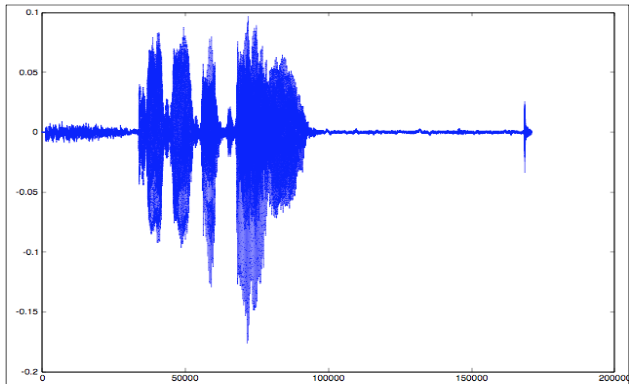
\includegraphics[width=9cm]{thesis/images/corr}\\
  \caption{Original waveform input for auto-correlation}\label{fig_c3_exp01}
\end{figure}

\subsubsection{Segmentation}
\textcolor{blue}{Generally, speech recognition preprocessing uses a fixed, overlapping window for segmentation. The segmentation algorithm designed for this experiment rather attempts to simulate and segment phoneme transitions using a natural phonetic  transition process between vowel (periodic signals) and consonants (non-periodic-noisy signals). Figure \ref{fig_c3_exp02} describes the various steps of the segmentation phase while Figure \ref{fig_c3_exp01} shows the original audio file. At the segmentation phase, we first of all adjust the scale of the original raw audio file to have only positive values rather than having it centred about the zero value on the x-axis (Figure \ref{fig_c3_exp02}a).  The pre-filtering removed all the negative signal values and retained only all the positive values.  At the next step, a smoothing kernel is selected based on experimentation to perform both smoothing as well as determining the peaks and trough (\ref{fig_c3_exp02}b).   The simple moving-average filter had a range of 5000 points and was used to extend the vowel regions so to make them more pronounced as well as smooth out the signal profile.    Then a threshold is applied to segment the waveform based on discovered inflection points (Figure \ref{fig_c3_exp02}c and d).  Segmentation can take place as the signal transitions between peaks and troughs in Figure \ref{fig_c3_exp02}.}

\begin{figure}
\centering
  % Requires \usepackage{graphicx}
  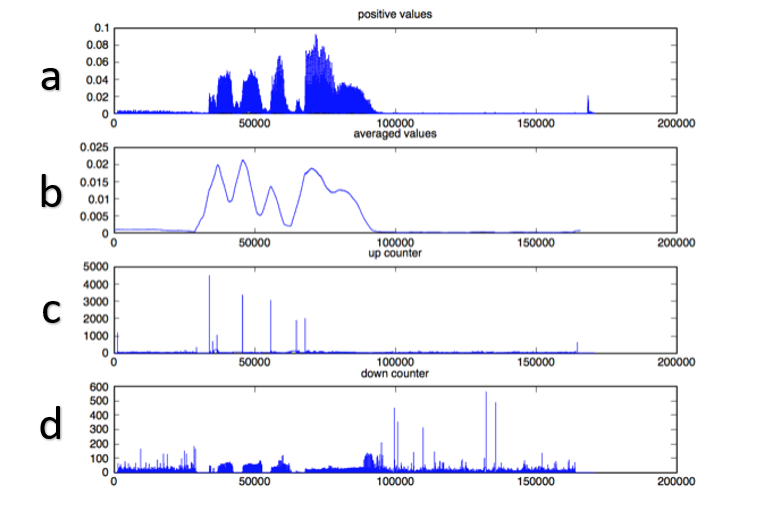
\includegraphics[width=9cm]{thesis/images/corr00}\\
  \caption{(a) Positive values of original waveform (b) Filtered values (c) Peak counter (d) Trough counter}\label{fig_c3_exp02}
\end{figure}
\subsubsection{Auto-correlation}
At the auto-correlation stage estimated phoneme segment boundaries are stored in an array and cross-correlated with the original signal.  Even though at a top-level view, the entire signal is auto-correlated, at the individual segment level, the signals are cross correlated against one another.  Furthermore, to achieve a ‘fair’ correlation estimate, individual segments representing estimated phonemes need to be re-sampled to eliminate mismatching of contour representations of the individual phonemes.\textcolor{blue}{  This was achieved by the filtering done at the segmentation stage.  Figure \ref{fig_c3_exp03} below shows sample auto-correlation result for the first peak-to-trough segment.}
\begin{figure}
\centering
  % Requires \usepackage{graphicx}
  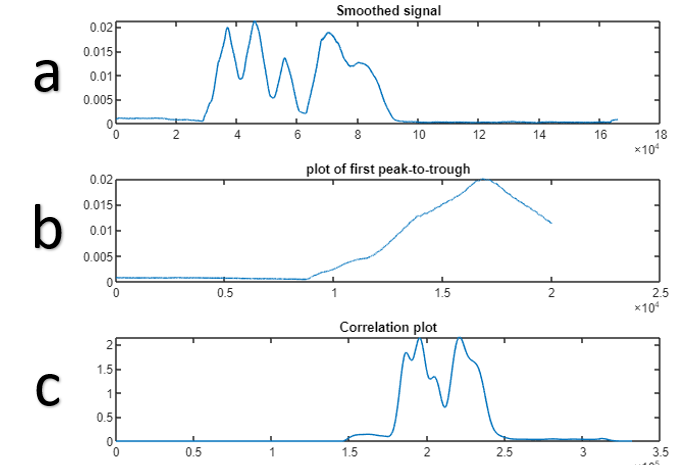
\includegraphics[width=9cm]{thesis/images/corr01}\\
  \caption{(a) Positive values of original waveform (b) Filtered values (c) Peak counter (d) Trough counter}\label{fig_c3_exp03}
\end{figure}

\startblue
Figure \ref{fig_c3_exp03}(a) is the smoothed signal from the segmentation procedure.  Figure \ref{fig_c3_exp03}(b) is the first peak to trough indicating the first phoneme in the utterance, and Figure \ref{fig_c3_exp03}(c) shows the autocorrelation plot.  From Figure \ref{fig_c3_exp03}(c), it can be seen from the twin peaks in the cross-correlation plot indicates that the phoneme-pair in the first peak-to-trough segment was discovered twice within the signal.  And this can form the basis of the phoneme's posterior distribution.  If there was a way of improving the accuracy of phoneme detection was not within the scope of this research.

The proposed auto-correlation algorithm performs both top-down and bottom-top processing.  In the first stage it does bottom-top segmentation, while in the second phase top-bottom auto-correlation.   The major weakness of this auto-correlation method is the lack of context between the phonemes.  For example consonants, which comprise non periodic noise signals, will be difficult to detect without the context of surrounding preceding and succeeding phonemes to the extent of a phrase-level of proximity context phonemes.  These contextual relationships can not be resolved in shallow systems such as this.  The Bayesian method of segmentation \citep{kamper2016unsupervised}, provides an alternative method which seeks to improve on these weaknesses using ASR feature preprocessing.  In this scheme, a combination of acoustic embedding and Dynamic Time Warping (DTW) for clustering is employed to replace auto-correlation.  In essence, it is beneficial to perform clustering on extracted features with less intrinsic noise than using an only smoothed audio data.\stopblue

\subsection{Experiments with Nao robot}
Nao is a humanoid robot developed mainly for deployment in environments for robotics education and development purposes.  Nao comes with a speech recognition software that offers features such as language settings and recognition sensitivity.  However it was understandably found to be limited because the Nao robot itself does not possess the processing power to perform CPU intensive training of acoustic models.  The Nao robot did however offer a level of support for using the pocketsphinx system. The pocketsphinx system is the C-language equivalent of CMUSphinx speech recognizer system also by Carnegie Mellon University.  Using the pocketsphinx method, acoustic models trained high performance systems can then be deployed to Nao for fast decoding within the Nao.  

\subsection{Digit Speech Recognition and Alignment Experiments}\label{sec_digitspeech}
These experiments were performed using CMU Sphinx4 recognition system and Kaldi speech recognition software.  While CMU Sphinx and pocketsphinx delivered standard interface for speech recognition using generative hybrid models, Kaldi speech in addition also offered advanced methods such as subspace Gaussian mixture model used to develop cross-lingual acoustic models and deep architectures for hybrid generative-discriminative models for speech recognition.   The main challenge with Kaldi was that it was CPU intensive and required a reasonable amount of parallel processing to achieve good results within a reasonable time period. 

Speech alignment experiments were performed using the Alisa \cite{stan2016alisa} tool which is a python based tool with calls made to the HMM toolkit \cite{young2002htk}.  The Alisa tool alignment process undergoes a semi-supervised process and requires an error prone time-intensive manual pre-alignment procedure.  The tool itself was found to be quite unstable and the output results were not very easily reproducible for further tests to be carried out on different data sets.  In addition, the time-intensive pre-alignment procedure made the tool not very useful for this research. Had the tool been more successful, the tool, which utilises \acrfull{vad} algorithms, would have been especially useful for sentence segmentation of long sequences of transcribed audio speech.  This tool however still lacked in alignment at either a word-level or sub-word level of alignment required in ASR pipelines.

\startblue
\section{Sequence-to-sequence Model Experiments}\label{sec_postalign}
A significant issue arises when using HMM-based toolkits such as Kaldi.  This is the requirement for aligned speech.  In more recent endeavours, there have been efforts towards automatic alignment of transcribed audio speech recordings through successive Baum-Welch estimation techniques \citep{gales2014speech,ragni2018automatic,ragni2014data}. However, this technique is not particularly compatible with end-to-end goals adopted for this research as it would require preprocessing and successive pre-training of the data set.

The following section introduces \acrshort{rnn} sequence-to-sequence modelling and some of the pilot studies done using these models and in Chapters \ref{ch6_speech} and \ref{ch8_future}, how these methods deal with the problem of automatic speech alignment in a fashion which is compatible with end-to-end speech processing.  The end-to-end requirements were desirable for low-resource speech recognition as it introduces a simpler speech model design.  The downside however to the end-to-end approach is the dependency on very deep recurrent neural network structures which require large volumes of data for successful training.

In the wild, three types of naturally occurring sequence relationships exist: the one-to-many relationship also referred to here as \acrfull{simo}; the many-to-one relationship also referred to here as \acrfull{miso}, and; the many-to-many also referred to here as \acrfull{mimo}.  The one-to-one relationship also referred to as \acrfull{siso} is excluded here.  Although the \acrshort{siso} relationship is a naturally existing relationship, this relationship is not sequential in nature and will not be modelled using a \acrlong{rnn}, but rather, can be modelled using regular \acrlong{dnn}s.  In addition, the \acrshort{mimo} relationship can be further subdivided into synchronous and asynchronous \acrshort{mimo}. In synchronous \acrshort{mimo}, the inputs and the outputs have equal lengths but in the asynchronous \acrshort{mimo}, the inputs and the outputs lengths are not necessarily equal.

\begin{figure}
\centering
  % Requires \usepackage{graphicx}
  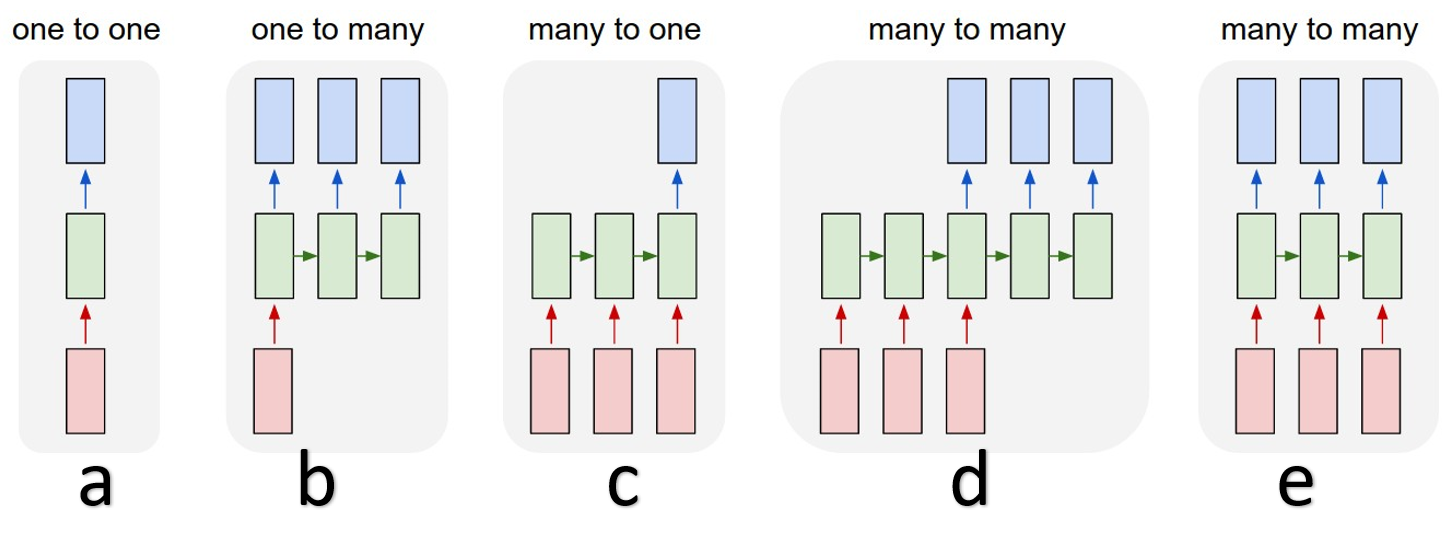
\includegraphics[width=9cm]{thesis/images/seq03.PNG}\\
  \caption{Types of Sequence-to-Sequence networks.  \citep{karpathy2015unreasonable}}\label{fig_c3_seq2seq}
\end{figure}

Figure \ref{fig_c3_seq2seq} illustrates how the five  relationship types are translated into neural networks where (\ref{fig_c3_seq2seq}a) refers to a regular \acrshort{dnn} structure and (\ref{fig_c3_seq2seq}b to d) are different \acrshort{rnn} structures. Examples of each type of relationship structure are given in \cite{karpathy2015unreasonable}.  An example of a \
\stopblue

\subsection{Tensor flow sequence-to-sequence character-to-diacritically-labelled-character model}\label{sec_c2d}
Experiments performed in this and the next three sections are all based on sequence-to-sequence modelling using recurrent neural networks.  While the this section and the next section represent precursor experiments centred around speech recognition tasks, the later two sections represent the final experiments reported in this work.

The character-to-diacritically labelled character model was a sequence-to-sequence diacritically labeled experiment to automatically infer diacritic transcriptions of the Wakirike language given the plain unmarked Wakirike language text as input.  This is a task, when achieved successfully, then becomes a sub task towards developing a phonetic dictionary for the Wakirike Language and the phonetic dictionary in turn can be used in HMM speech recognition or equivalent  end-to-end models.  This experiment was a precursor experiment, the results of which were reserved for further study.

\subsection{Sequence-to-sequence Grapheme-to-Phoneme (G2P) model}\label{sec_c3_g2p}
This follow up experiment to the previous experiment in section \ref{sec_c2d},  attempts to automatically generate a phonetic dictionary from graphemes in a text corpus. Grapheme-to-phoneme experiments come in two flavours, the first being a continuation of the previous experiment, that is, using diacritically marked symbols, and the second flavour using non-marked graphemes as input.  The experiments we performed used the latter non-marked graphemes as input. As this experiment was also a subtask in HMM speech model building,  the results of these experiments were reserved for further study.

What follows in the next three sections are sequence-to-sequence experiments actively developed in this research and are detailed in chapters (\ref{ch6_wlm},\ref{ch6_speech} and \ref{ch8_future}).  A brief summary of the experiments are highlighted in the following sections (\ref{sec_grulm}, \ref{sec_be2e} and \ref{c3sec_espnet}).  Note that these models all utilise TensorFlow deep learning library including the Bi-directional speech model (section \ref{sec_be2e}) which is built on top of Mozilla DeepSpeech with the exception of section \ref{c3sec_espnet} which is based on PyTorch; a similar deep learning library.

\subsection{GRU language model for Wakirike language based on TensorFlow}\label{sec_grulm}
The language model developed in this research is a character-based sequence-to-sequence deep recurrent neural network that maps a sequence of characters to a sequence of words found in the training data set. This model met the objective of reducing the vocabulary size required for language models as well as the text corpus required as inferences could be made over the smaller-fixed character vocabulary rather than orders or magnitude larger word corpus with the possibility of out of vocabulary terms found in the training data.  Though this may occur in the character sequence-model at the inference stage, it would not normally happen during training.  The neural network model developed is described in Chapters \ref{ch3RNN} and \ref{ch6_speech}, and consists of Gated Recurrent Unit (GRU) Recurrent Neural Network (RNN). The GRU is a specialised type of Long Short-Term Memory (LSTM) cell RNN.  The emphasis here is on the ability to model over particularly long sequences of the training data.  In this case, over long character sequences.  Thus, the network is able to learn long term dependencies as would be naturally required to construct grammatically correct sentences.  In essence, the RNN is able to learn grammar rules inherently from the training data.

\subsection{Bi-Directional LSTM-based end-to-end speech model}\label{sec_be2e}
A similar LSTM sequence-to-sequence network based on Baidu Research’s original research design \citep{hannun2014deep} is developed in this research for end-to-end speech recognition.  This model, as its name implies, attempts to establish long term relationships by adding a reinforcing LSTM layer learning information but this time from the opposite direction, hence the bi-directional architecture.  

In addition, the model incorporates the Connectionist Temporal Classifier (CTC) decoder. This enables the model to make run-time inferences on both the character as well as estimate audio wave to character label alignment simultaneously.  This makes this design accommodate end-to-end goals and ultimately simplifies the overall design and completely eliminates the need for either manual or semi-supervised alignments mentioned previously in sections (\ref{sec_c3_alisa}, \ref{sec_digitspeech} and \ref{sec_postalign}).

\subsection{ESP-Net Experiments}\label{c3sec_espnet}
The ESP-Net (End-to-end Speech Network) toolkit \citep{watanabe2018espnet}, is a speech processing toolkit that was of interest to this research because it offers end-to-end capabilities not only in \acrfull{asr} but also in \acrfull{tts} or speech synthesis and other speech-sequence-processing related tasks.  In addition, the toolkit offers multi-modal training combining both Attention networks \cite{vaswani2017attention} with CTC Transformer networks as well as multi-channel feature representation that is, the fusing together of multiple feature representations of an audio signal.

\section{Method of evaluation}
System building methodology \citep{nunamaker1990systems} for speech recognition systems requires models to be evaluated against speech recognition Machine Learning metrics.  For language models, perplexity metric was used for evaluation.  \acrfull{bleu}\citep{papineni2002bleu} has also been used as a metric for evaluating language models.

Perplexity measures the complexity of a language that the language model is designed to represent \citep{1976jelinekcontinuous}. In practice, the entropy of a language with an N-gram language model $P_N(W)$ is measured from a set of sentences and is defined as
\begin{equation}H=\sum_{\mathbf{W}\in\Omega}P_N(\mathbf{W})
\label{eqn_c2_lm05}
\end{equation}

where $\Omega$ is a set of sentences of the language. The perplexity, which is interpreted as the average word-branching factor, is defined as
\begin{equation}PP(W)=2^H
\label{eqn_c2_lm06}
\end{equation}
where H is the average entropy of the system or the average log probability defined as
\begin{equation}
H=-\frac{1}{N}\sum_{i=1}^N[log_2P(w_1,w_2\dots w_N)]
\label{eqn_c2_lm07}
\end{equation}
For a bi gram model therefore, equation (\ref{eqn_c2_lm07}) becomes
\begin{equation}
PP(W)=2^H=2^{-\frac{1}{N}\sum_{i=1}^N[log_2P(w_1,w_2\dots w_N)]}
\label{eqn_c2_lm08}
\end{equation}
After simplifying we have
\begin{equation}
PP(W)=\sqrt[N]{\prod_{i=1}^N\frac{1}{P(w_i|w_{i-1})}}
\label{eqn_c2_lm09}
\end{equation}


Full speech recognition pipelines are usually evaluated against the Word Error Rate (WER).  WER is computed as follows:
\begin{equation}\label{eqn_2_3_wer}
WER=\frac{I+D+R}{WC}\times 100
\end{equation}
Here $I,D,$ and $R$ are wrong insertions, deletions and replacements respectively and $WC$ is the word count.

Metrics used for low speech recognition in the zero speech challenge \citep{versteegh2015zero} include the ABX metric. Other common speech recognition error metrics following a similar definition as the Word Error Rate (WER) are Character Error Rate (CER), Phoneme Error Rate (PER) and Syllabic Error Rate (SyER) and sentence error rate (SER).

\section{Chapter Summary}
In this chapter we outline how this research set out to achieve its objectives.  The main claim of this research is that by building a speech model that combines knowledge of end-to-end processing along with state of the art signal processing, the overall training complexity and build time for new ASR systems can be improved.  This research aims to deliver this through by the unique combination of a CTC-based deep recurrent bi-directional neural network with high performance feature processing of Deep Scattering Networks (DSNs).

This chapter also reviews the technologies utilised by this research in order to arrive at the research outputs and briefly describes the experiments performed.  Within this space we describe CMUSphinx, Kaldi, Mozilla DeepSpeech, TensorFlow, Matlab and ScatNet as major libraries used.   The first two of these are Hidden Markov Model (HMM)-based libraries and the rest are  signal processing systems used to build Deep Recurrent Neural Network (RNN) models. Finally, we mention metrics for the evaluation of the models built in this research.
